\documentclass{article} %standalone
\usepackage{tikz}
\usepackage[left=0.1cm, right=0.1cm]{geometry}
\begin{document}


\begin{figure}[t]
\resizebox{\columnwidth}{!}{%


% INSERT HERE THE OUTPUT OF "bunx aos-sched export complete/blank"

% EXAMPLE":
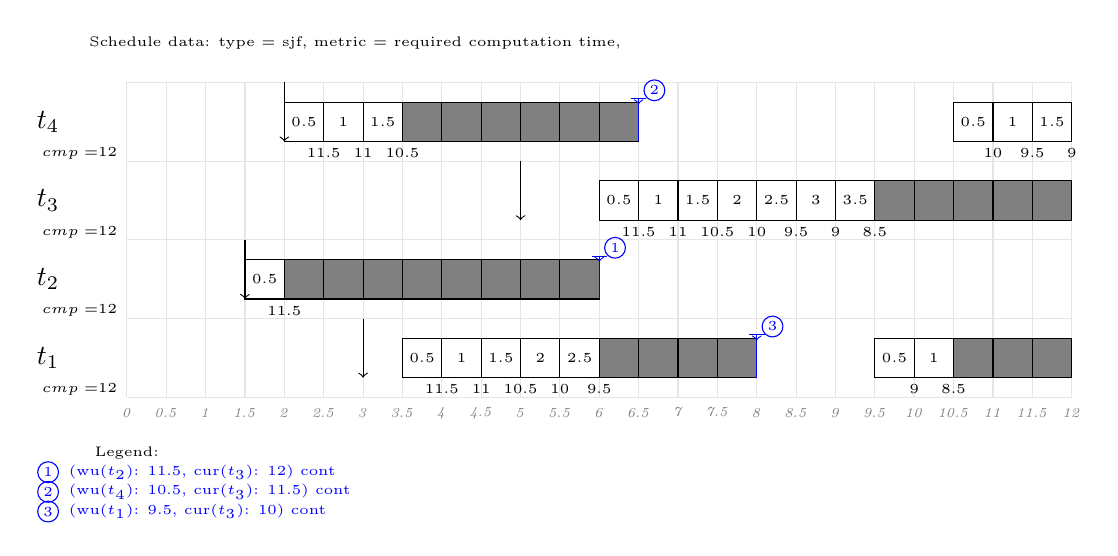
\begin{tikzpicture}
\draw[xstep=0.5,gray!20,thin,shift={(0,-0.25)}] (0,0) grid (12,4);
\node [text=gray] at(0, -0.44999999999999996) {\tiny \emph{0}};
\node [text=gray] at(0.5, -0.44999999999999996) {\tiny \emph{0.5}};
\node [text=gray] at(1, -0.44999999999999996) {\tiny \emph{1}};
\node [text=gray] at(1.5, -0.44999999999999996) {\tiny \emph{1.5}};
\node [text=gray] at(2, -0.44999999999999996) {\tiny \emph{2}};
\node [text=gray] at(2.5, -0.44999999999999996) {\tiny \emph{2.5}};
\node [text=gray] at(3, -0.44999999999999996) {\tiny \emph{3}};
\node [text=gray] at(3.5, -0.44999999999999996) {\tiny \emph{3.5}};
\node [text=gray] at(4, -0.44999999999999996) {\tiny \emph{4}};
\node [text=gray] at(4.5, -0.44999999999999996) {\tiny \emph{4.5}};
\node [text=gray] at(5, -0.44999999999999996) {\tiny \emph{5}};
\node [text=gray] at(5.5, -0.44999999999999996) {\tiny \emph{5.5}};
\node [text=gray] at(6, -0.44999999999999996) {\tiny \emph{6}};
\node [text=gray] at(6.5, -0.44999999999999996) {\tiny \emph{6.5}};
\node [text=gray] at(7, -0.44999999999999996) {\tiny \emph{7}};
\node [text=gray] at(7.5, -0.44999999999999996) {\tiny \emph{7.5}};
\node [text=gray] at(8, -0.44999999999999996) {\tiny \emph{8}};
\node [text=gray] at(8.5, -0.44999999999999996) {\tiny \emph{8.5}};
\node [text=gray] at(9, -0.44999999999999996) {\tiny \emph{9}};
\node [text=gray] at(9.5, -0.44999999999999996) {\tiny \emph{9.5}};
\node [text=gray] at(10, -0.44999999999999996) {\tiny \emph{10}};
\node [text=gray] at(10.5, -0.44999999999999996) {\tiny \emph{10.5}};
\node [text=gray] at(11, -0.44999999999999996) {\tiny \emph{11}};
\node [text=gray] at(11.5, -0.44999999999999996) {\tiny \emph{11.5}};
\node [text=gray] at(12, -0.44999999999999996) {\tiny \emph{12}};
\node at(-1, 0.25) {$t_1$};
\node at(-1, 1.25) {$t_2$};
\node at(-1, 2.25) {$t_3$};
\node at(-1, 3.25) {$t_4$};
\node at(-0.6, -0.15000000000000002) {\tiny $cmp=$12};
\node at(-0.6, 0.04999999999999999) {\tiny };
\node at(-0.6, 0.85) {\tiny $cmp=$12};
\node at(-0.6, 1.05) {\tiny };
\node at(-0.6, 1.85) {\tiny $cmp=$12};
\node at(-0.6, 2.05) {\tiny };
\node at(-0.6, 2.85) {\tiny $cmp=$12};
\node at(-0.6, 3.05) {\tiny };
\draw[draw=black] (1.5, 1) rectangle ++(0.5,0.5) node[pos=.5] {};
\node at(2, 0.85) {\tiny 11.5};
\node at(1.75, 1.25) {\tiny $0.5$};
\draw[draw=black, fill=gray] (2, 1) rectangle ++(0.5,0.5) node[pos=.5, text=white] {};
\draw[draw=black] (2, 3) rectangle ++(0.5,0.5) node[pos=.5] {};
\node at(2.5, 2.85) {\tiny 11.5};
\node at(2.25, 3.25) {\tiny $0.5$};
\draw[draw=black, fill=gray] (2.5, 1) rectangle ++(0.5,0.5) node[pos=.5, text=white] {};
\draw[draw=black] (2.5, 3) rectangle ++(0.5,0.5) node[pos=.5] {};
\node at(3, 2.85) {\tiny 11};
\node at(2.75, 3.25) {\tiny $1$};
\draw[draw=black, fill=gray] (3, 1) rectangle ++(0.5,0.5) node[pos=.5, text=white] {};
\draw[draw=black] (3, 3) rectangle ++(0.5,0.5) node[pos=.5] {};
\node at(3.5, 2.85) {\tiny 10.5};
\node at(3.25, 3.25) {\tiny $1.5$};
\draw[draw=black] (3.5, 0) rectangle ++(0.5,0.5) node[pos=.5] {};
\node at(4, -0.15000000000000002) {\tiny 11.5};
\node at(3.75, 0.25) {\tiny $0.5$};
\draw[draw=black, fill=gray] (3.5, 1) rectangle ++(0.5,0.5) node[pos=.5, text=white] {};
\draw[draw=black, fill=gray] (3.5, 3) rectangle ++(0.5,0.5) node[pos=.5, text=white] {};
\draw[draw=black] (4, 0) rectangle ++(0.5,0.5) node[pos=.5] {};
\node at(4.5, -0.15000000000000002) {\tiny 11};
\node at(4.25, 0.25) {\tiny $1$};
\draw[draw=black, fill=gray] (4, 1) rectangle ++(0.5,0.5) node[pos=.5, text=white] {};
\draw[draw=black, fill=gray] (4, 3) rectangle ++(0.5,0.5) node[pos=.5, text=white] {};
\draw[draw=black] (4.5, 0) rectangle ++(0.5,0.5) node[pos=.5] {};
\node at(5, -0.15000000000000002) {\tiny 10.5};
\node at(4.75, 0.25) {\tiny $1.5$};
\draw[draw=black, fill=gray] (4.5, 1) rectangle ++(0.5,0.5) node[pos=.5, text=white] {};
\draw[draw=black, fill=gray] (4.5, 3) rectangle ++(0.5,0.5) node[pos=.5, text=white] {};
\draw[draw=black] (5, 0) rectangle ++(0.5,0.5) node[pos=.5] {};
\node at(5.5, -0.15000000000000002) {\tiny 10};
\node at(5.25, 0.25) {\tiny $2$};
\draw[draw=black, fill=gray] (5, 1) rectangle ++(0.5,0.5) node[pos=.5, text=white] {};
\draw[draw=black, fill=gray] (5, 3) rectangle ++(0.5,0.5) node[pos=.5, text=white] {};
\draw[draw=black] (5.5, 0) rectangle ++(0.5,0.5) node[pos=.5] {};
\node at(6, -0.15000000000000002) {\tiny 9.5};
\node at(5.75, 0.25) {\tiny $2.5$};
\draw[draw=black, fill=gray] (5.5, 1) rectangle ++(0.5,0.5) node[pos=.5, text=white] {};
\draw[draw=black, fill=gray] (5.5, 3) rectangle ++(0.5,0.5) node[pos=.5, text=white] {};
\draw[draw=black, fill=gray] (6, 0) rectangle ++(0.5,0.5) node[pos=.5, text=white] {};
\node [shape=circle,draw, inner sep=1pt, blue]
          at(6.2, 1.65) {\tiny 1};
\draw[draw=blue] [|>-] (6, 1 + 0.55) -- (6, 1);
\draw[draw=black] (6, 2) rectangle ++(0.5,0.5) node[pos=.5] {};
\node at(6.5, 1.85) {\tiny 11.5};
\node at(6.25, 2.25) {\tiny $0.5$};
\draw[draw=black, fill=gray] (6, 3) rectangle ++(0.5,0.5) node[pos=.5, text=white] {};
\draw[draw=black, fill=gray] (6.5, 0) rectangle ++(0.5,0.5) node[pos=.5, text=white] {};
\draw[draw=black] (6.5, 2) rectangle ++(0.5,0.5) node[pos=.5] {};
\node at(7, 1.85) {\tiny 11};
\node at(6.75, 2.25) {\tiny $1$};
\node [shape=circle,draw, inner sep=1pt, blue]
          at(6.7, 3.65) {\tiny 2};
\draw[draw=blue] [|>-] (6.5, 3 + 0.55) -- (6.5, 3);
\draw[draw=black, fill=gray] (7, 0) rectangle ++(0.5,0.5) node[pos=.5, text=white] {};
\draw[draw=black] (7, 2) rectangle ++(0.5,0.5) node[pos=.5] {};
\node at(7.5, 1.85) {\tiny 10.5};
\node at(7.25, 2.25) {\tiny $1.5$};
\draw[draw=black, fill=gray] (7.5, 0) rectangle ++(0.5,0.5) node[pos=.5, text=white] {};
\draw[draw=black] (7.5, 2) rectangle ++(0.5,0.5) node[pos=.5] {};
\node at(8, 1.85) {\tiny 10};
\node at(7.75, 2.25) {\tiny $2$};
\node [shape=circle,draw, inner sep=1pt, blue]
          at(8.2, 0.65) {\tiny 3};
\draw[draw=blue] [|>-] (8, 0 + 0.55) -- (8, 0);
\draw[draw=black] (8, 2) rectangle ++(0.5,0.5) node[pos=.5] {};
\node at(8.5, 1.85) {\tiny 9.5};
\node at(8.25, 2.25) {\tiny $2.5$};
\draw[draw=black] (8.5, 2) rectangle ++(0.5,0.5) node[pos=.5] {};
\node at(9, 1.85) {\tiny 9};
\node at(8.75, 2.25) {\tiny $3$};
\draw[draw=black] (9, 2) rectangle ++(0.5,0.5) node[pos=.5] {};
\node at(9.5, 1.85) {\tiny 8.5};
\node at(9.25, 2.25) {\tiny $3.5$};
\draw[draw=black] (9.5, 0) rectangle ++(0.5,0.5) node[pos=.5] {};
\node at(10, -0.15000000000000002) {\tiny 9};
\node at(9.75, 0.25) {\tiny $0.5$};
\draw[draw=black, fill=gray] (9.5, 2) rectangle ++(0.5,0.5) node[pos=.5, text=white] {};
\draw[draw=black] (10, 0) rectangle ++(0.5,0.5) node[pos=.5] {};
\node at(10.5, -0.15000000000000002) {\tiny 8.5};
\node at(10.25, 0.25) {\tiny $1$};
\draw[draw=black, fill=gray] (10, 2) rectangle ++(0.5,0.5) node[pos=.5, text=white] {};
\draw[draw=black, fill=gray] (10.5, 0) rectangle ++(0.5,0.5) node[pos=.5, text=white] {};
\draw[draw=black, fill=gray] (10.5, 2) rectangle ++(0.5,0.5) node[pos=.5, text=white] {};
\draw[draw=black] (10.5, 3) rectangle ++(0.5,0.5) node[pos=.5] {};
\node at(11, 2.85) {\tiny 10};
\node at(10.75, 3.25) {\tiny $0.5$};
\draw[draw=black, fill=gray] (11, 0) rectangle ++(0.5,0.5) node[pos=.5, text=white] {};
\draw[draw=black, fill=gray] (11, 2) rectangle ++(0.5,0.5) node[pos=.5, text=white] {};
\draw[draw=black] (11, 3) rectangle ++(0.5,0.5) node[pos=.5] {};
\node at(11.5, 2.85) {\tiny 9.5};
\node at(11.25, 3.25) {\tiny $1$};
\draw[draw=black, fill=gray] (11.5, 0) rectangle ++(0.5,0.5) node[pos=.5, text=white] {};
\draw[draw=black, fill=gray] (11.5, 2) rectangle ++(0.5,0.5) node[pos=.5, text=white] {};
\draw[draw=black] (11.5, 3) rectangle ++(0.5,0.5) node[pos=.5] {};
\node at(12, 2.85) {\tiny 9};
\node at(11.75, 3.25) {\tiny $1.5$};
\draw [->] (3, 0 + 0.75) -- (3, 0);
\draw [->] (1.5, 1 + 0.75) -- (1.5, 1);
\draw [->] (5, 2 + 0.75) -- (5, 2);
\draw [->] (2, 3 + 0.75) -- (2, 3);
\node [anchor=west] at(-0.6, 4.25) {\tiny Schedule data: type = sjf, metric = required computation time, };
\node [shape=circle, draw, inner sep=1pt, blue] (legendNode0) at(-1, -1.2) {\tiny 1};
    \node [right, text=blue] at(legendNode0.east) {\tiny (wu($t_2$): 11.5, cur($t_3$): 12) cont};
\node [shape=circle, draw, inner sep=1pt, blue] (legendNode1) at(-1, -1.45) {\tiny 2};
    \node [right, text=blue] at(legendNode1.east) {\tiny (wu($t_4$): 10.5, cur($t_3$): 11.5) cont};
\node [shape=circle, draw, inner sep=1pt, blue] (legendNode2) at(-1, -1.7) {\tiny 3};
    \node [right, text=blue] at(legendNode2.east) {\tiny (wu($t_1$): 9.5, cur($t_3$): 10) cont};
\node [below] at(0, -0.75) {\tiny Legend:};
\end{tikzpicture}





}
\end{figure}







% INSERT HERE THE OUTPUT OF "bunx aos-sched export data" AND/OR "bunx aos-sched table complete/blank"

% EXAMPLE":
Schedule data: type = sjf, metric = required computation time,
\begin{itemize}
\item task $t_1$ (cmp = 12) arrives at 3, runs for 2.5, waits for 2, runs for 1, waits for 3, runs for 2
\item task $t_2$ (cmp = 12) arrives at 1.5, runs for 0.5, waits for 4, runs for 2.5, waits for 1, runs for 2.5
\item task $t_3$ (cmp = 12) arrives at 5, runs for 3.5, waits for 4, runs for 4, waits for 3.5, runs for 4
\item task $t_4$ (cmp = 12) arrives at 2, runs for 1.5, waits for 3, runs for 3.5, waits for 1.5, runs for 3
\end{itemize}

\begin{table}[]
\centering
\caption{Summary of Tasks}
\vspace{10pt}
\begin{tabular}{c|c|c|c|c|c|c}
Task & Arrival & Computation & Start & Finish & Waiting (W) & Turnaround (Z) \\
\hline
1 & 3 & 12 & 3.5 &  & 2 &  \\
2 & 1.5 & 12 & 1.5 &  & 6 &  \\
3 & 5 & 12 & 6 &  & 1 &  \\
4 & 2 & 12 & 2 &  & 4 &  \\
\end{tabular}
\label{tab:my_label}
\end{table}




\end{document}